\documentclass[a4paper,man,floatsintext,donotrepeattitle]{apa6}

\usepackage{setspace}

\title{How Response Times Should Inform Test Assembly: A Note on the Speed Sensitivity Parameter in Response Time Modeling
\vspace{3cm}}
\shorttitle{Response Time Models in Test Assembly}

% Author information


\threeauthors{Benjamin Becker and Sebastian Weirich} {Dries Debeer} {Frank Goldhammer}
\threeaffiliations{Institute for Educational Quality Improvement} {University of Zurich} {DIPF | Leibniz Institute for Research and Information in Education \\
Centre for International Student Assessment (ZIB)}

\authornote{\textbf{Corresponding Author} \\

{\setstretch{1.0}Benjamin Becker \\ Institute for Educational Quality Improvement \\ Humboldt University Berlin \\
Unter den Linden 6, 10099 Berlin, Germany
 \\ +49 30  2093 46592 \\ b.becker@iqb.hu-berlin.de \\
}}

\begin{document}
%\maketitle

\pagenumbering{arabic}
\clearpage
\setcounter{page}{23}

\begin{table}[ht]
\centering
\caption{Means of the Posterior Distribution of Mean and Standard Deviation of the Item Parameters and the Correlations Between Item Parameters, j = 12.} 
\begin{tabular}{lrrlllll}
  \hline
Parameter & M & SD & $b_{k}$ & $a_{k}$ & $\lambda_{k}$ & $\phi_{k}$  \\ 
  \hline
$b_{k}$ & 0.54 & 1.89 &  &  &  &  \\ 
  $a_{k}$ & 1.12 & 0.66 & 0.07 &  &  &   \\ 
  $\lambda_{k}$ & 4.26 & 0.52 & 0.25 & 0.27 &  &   \\ 
  $\phi_{k}$ & 0.40 & 0.34 & -0.05 & 0.12 & 0.21 &   \\ 
   \hline
\end{tabular}
\label{tab:postMeans}
\end{table}
 
\vspace{4cm} 
 
\begin{table}[!htb]
\centering
\caption{Test Statistics per Test Form and per Speed Group, Averaged Across All Replications.} 
\begin{tabular}{llrrrrrr}
  \hline
Test Form & $\zeta_{i}$ & $M(RT_{tot})$ & $SD(RT_{tot})$ & $M(Mis)$ & $SD(Mis)$ & $cor(\theta_{true} \theta_{est})$ & RMSE \\ 
  \hline
low $\phi$ & slowest & 3634.74 & 367.96 & 0.02 & 0.04 & 0.90 & 0.47 \\ 
  low $\phi$ & slow & 3100.20 & 312.82 & 0.00 & 0.01 & 0.91 & 0.45 \\ 
  low $\phi$ & fast & 2273.33 & 227.33 & 0.00 & 0.00 & 0.91 & 0.45 \\ 
  low $\phi$ & fastest & 1954.34 & 196.28 & 0.00 & 0.00 & 0.91 & 0.45 \\ 
  high $\phi$ & slowest & 5419.48 & 551.18 & 0.30 & 0.09 & 0.82 & 0.84 \\ 
  high $\phi$ & slow & 3785.80 & 382.40 & 0.03 & 0.06 & 0.90 & 0.48 \\ 
  high $\phi$ & fast & 1861.38 & 186.27 & 0.00 & 0.00 & 0.91 & 0.45 \\ 
  high $\phi$ & fastest & 1309.45 & 131.00 & 0.00 & 0.00 & 0.91 & 0.45 \\ 
   \hline
\end{tabular}
\begin{tablenotes}
\vspace{0.1cm}
\small
    \textit{Note:} Descriptive statistics are depicted for mean response times M($RT_{tot}$) and the corresponding standard deviation SD($RT_{tot}$), mean amount of missings M(Mis), the corresponding standard deviation SD(Mis), correlation between true and estimated ability $cor(\theta_{true} \theta_{est})$ and root mean square error (RMSE). 
\end{tablenotes}
\label{tab:descr}
\end{table}

\begin{figure} [htb]
	\begin{center}
	 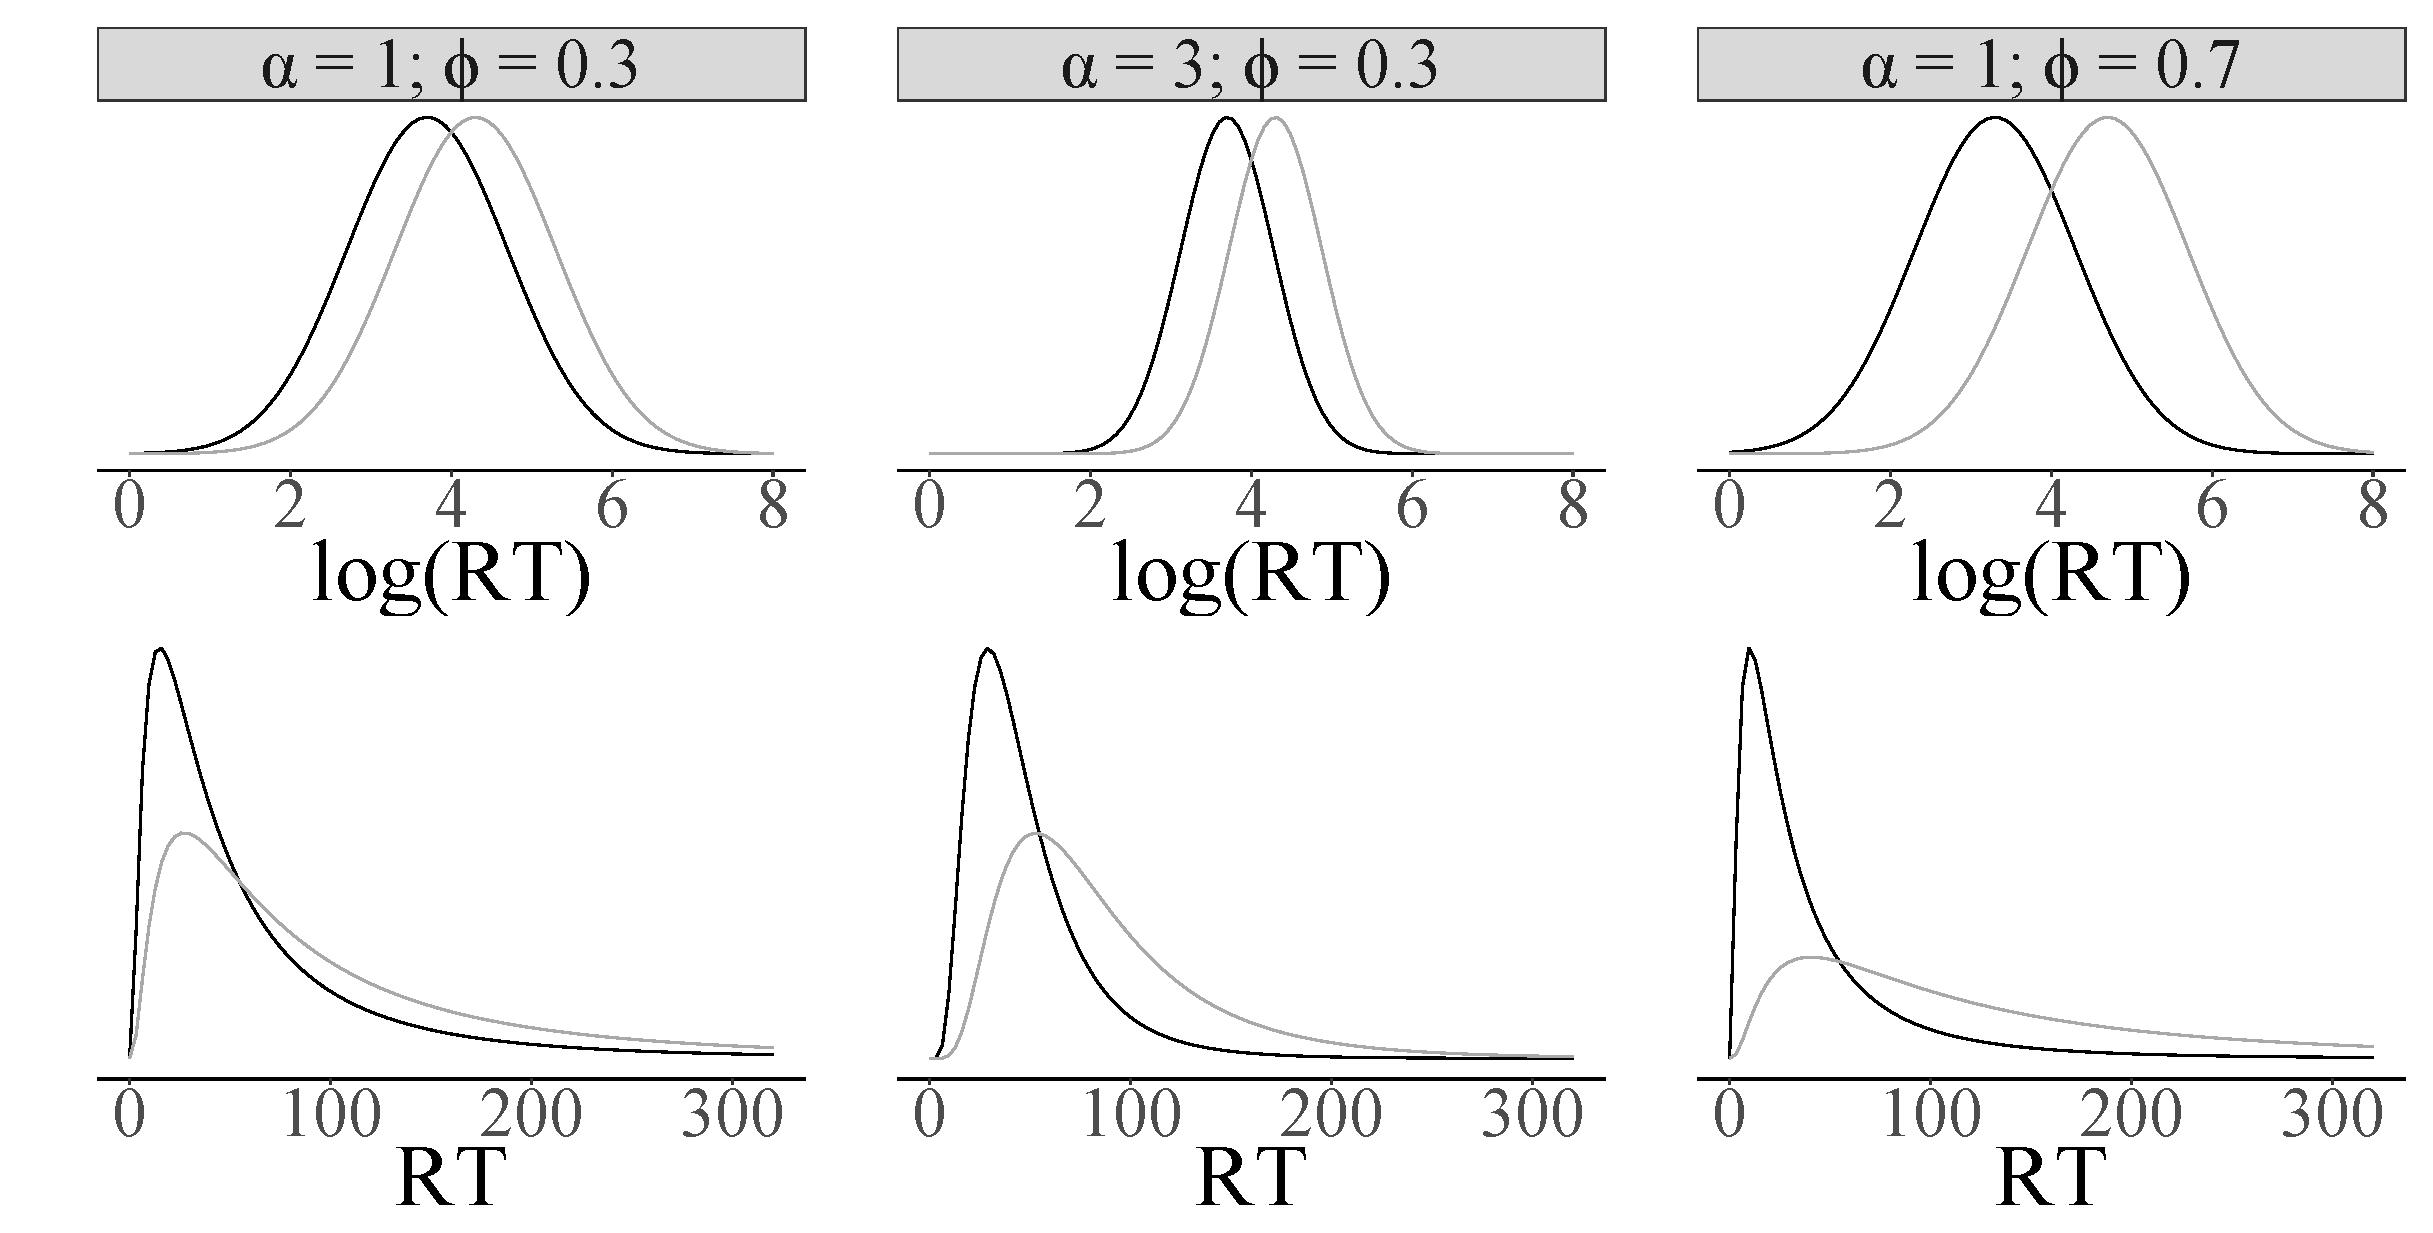
\includegraphics[height = 0.30\textheight]{discrimination_comp.eps}
	\end{center}		
	 \caption{Expected log response time (upper row) and response time (lower row) distributions of a fast person with $\zeta_1 = 1$ (black line) and a slow person with $\zeta_2 = -1$ (grey line) on three different items, all with $\lambda_k = 4$.} 
	 \label{fig:discr_diff}
\end{figure}


\begin{figure} [!htb]	
	\begin{center}
		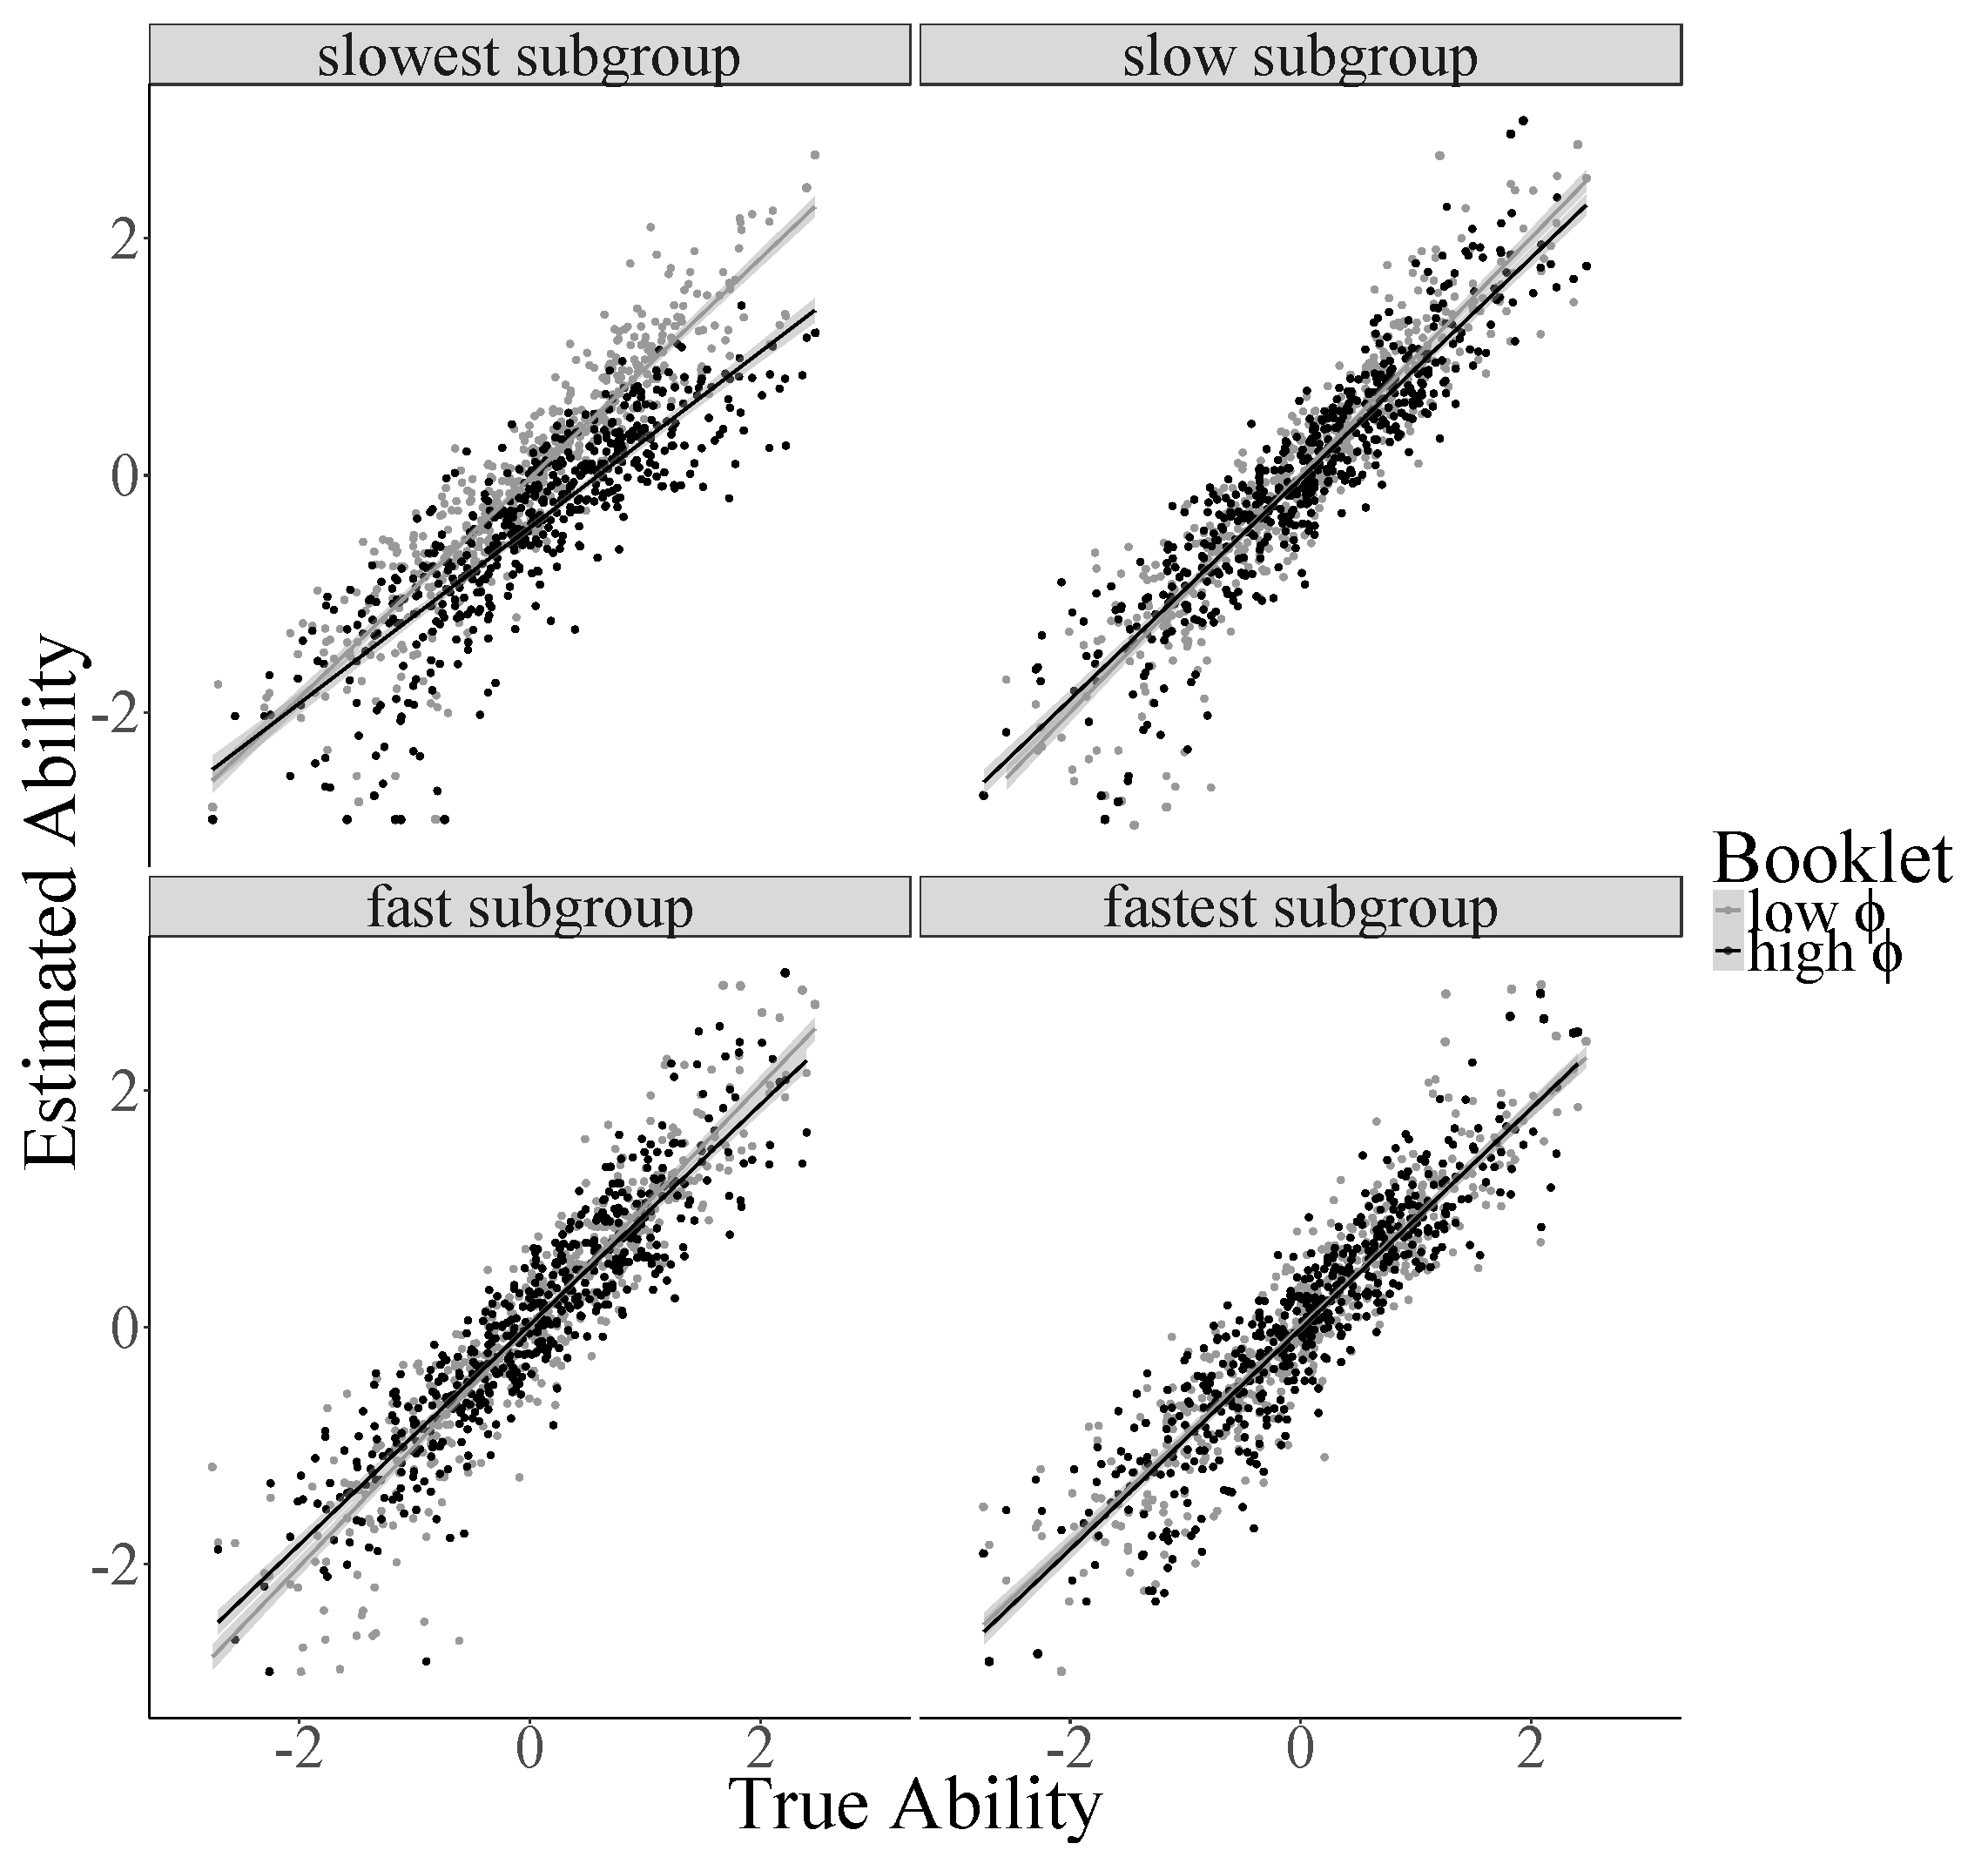
\includegraphics[height = 0.4\textheight]{abil_subGroup.eps}
	\end{center}
		\caption{True and estimated ability for the low and high speed sensitivity test form, across the four subgroups. Results shown for a randomly selected single replication.}	
		\label{fig:abil}
\end{figure}



\end{document}